\begin{resumo}
As enchentes urbanas estão entre os maiores desafios de cidades costeiras como o Recife. Fatores naturais — relevo plano, baixa altitude e influência das marés — somam-se a problemas causados pela ação humana, como a impermeabilização do solo e as ocupações irregulares. Esse conjunto de condições torna a capital pernambucana altamente vulnerável a alagamentos, que afetam milhares de pessoas todos os anos e geram prejuízos significativos à infraestrutura e à economia local.

Este trabalho apresenta o \textbf{FloodAI-Recife}, um sistema inteligente de previsão e monitoramento em tempo real de alagamentos urbanos. A solução integra dados meteorológicos fornecidos pela API da Agência Pernambucana de Águas e Clima (APAC), séries históricas de ocorrências e informações geoespaciais de áreas vulneráveis. O modelo preditivo adota uma abordagem híbrida, combinando análise estatística, aprendizado de máquina e classificação fuzzy para estimar o risco de alagamento em diferentes regiões da cidade.

O sistema oferece funcionalidades como: (i) \textbf{monitoramento em tempo real}, com atualização a cada 5 minutos; (ii) \textbf{previsão de risco}, atingindo 82\% de acurácia em comparação com registros da Defesa Civil; (iii) \textbf{visualização georreferenciada}, por meio de mapas interativos que exibem níveis de risco por bairro; e (iv) \textbf{alertas multicanais}, enviados via SMS, WhatsApp e notificações push, ampliando o alcance da informação preventiva.

Os resultados mostram que o FloodAI-Recife atende aos requisitos de desempenho e disponibilidade, com tempo médio de resposta de 1,2 segundos e disponibilidade de 99,8\%. O estudo de caso mapeou sete zonas críticas, abrangendo 28 bairros e 28 pontos de risco. Apesar dos avanços, o sistema ainda enfrenta limitações, como a dependência da qualidade dos dados da APAC e a cobertura restrita de estações meteorológicas. Como perspectivas futuras, destacam-se a integração de sensores IoT, o uso de modelos de aprendizado profundo e a expansão da solução para outras cidades brasileiras.

Em síntese, o FloodAI-Recife representa uma contribuição prática e inovadora para a gestão de riscos urbanos, oferecendo uma ferramenta acessível, escalável e de impacto social direto, capaz de apoiar tanto a população quanto os órgãos de defesa civil na mitigação dos efeitos dos alagamentos.
\end{resumo}

\section{Estudo de Caso: Recife}

\subsection{Áreas de Risco Mapeadas}

Foram identificadas sete zonas críticas, abrangendo 28 bairros. A Tabela~\ref{tab:areas-mapeadas} apresenta a distribuição de pontos de alagamento em cada área.

\begin{table}[H]
  \centering
  \caption{Áreas de Risco Mapeadas no Recife}
  \label{tab:areas-mapeadas}
  \begin{tabular}{p{0.4\linewidth}  c  c}
    \toprule
    \textbf{Zona}                       & \textbf{Bairros} & \textbf{Pontos Críticos} \\
    \midrule
    Zona Sul (Imbiribeira/Ipsep)        & 4                & 5                        \\
    Centro (Boa Vista/Santo Amaro)      & 4                & 5                        \\
    Zona Norte (Dois Irmãos)            & 4                & 4                        \\
    Zona Oeste (Várzea/Afogados)        & 4                & 4                        \\
    Centro Histórico                    & 3                & 4                        \\
    Zona Sul (Ibura/Jordão)             & 4                & 3                        \\
    Norte (Água Fria/Beberibe)          & 5                & 3                        \\
    \midrule
    \textbf{Total}                      & \textbf{28}      & \textbf{28}             \\
    \bottomrule
  \end{tabular}
\end{table}

\subsection{Dashboard do Sistema}

Para apoiar a análise e a tomada de decisão, o FloodAI-Recife disponibiliza um \textbf{dashboard interativo}, que reúne em um só lugar os principais indicadores de risco, mapas georreferenciados e alertas em tempo real. A seguir, são apresentadas algumas telas do sistema:

\begin{figure}[H]
  \centering
  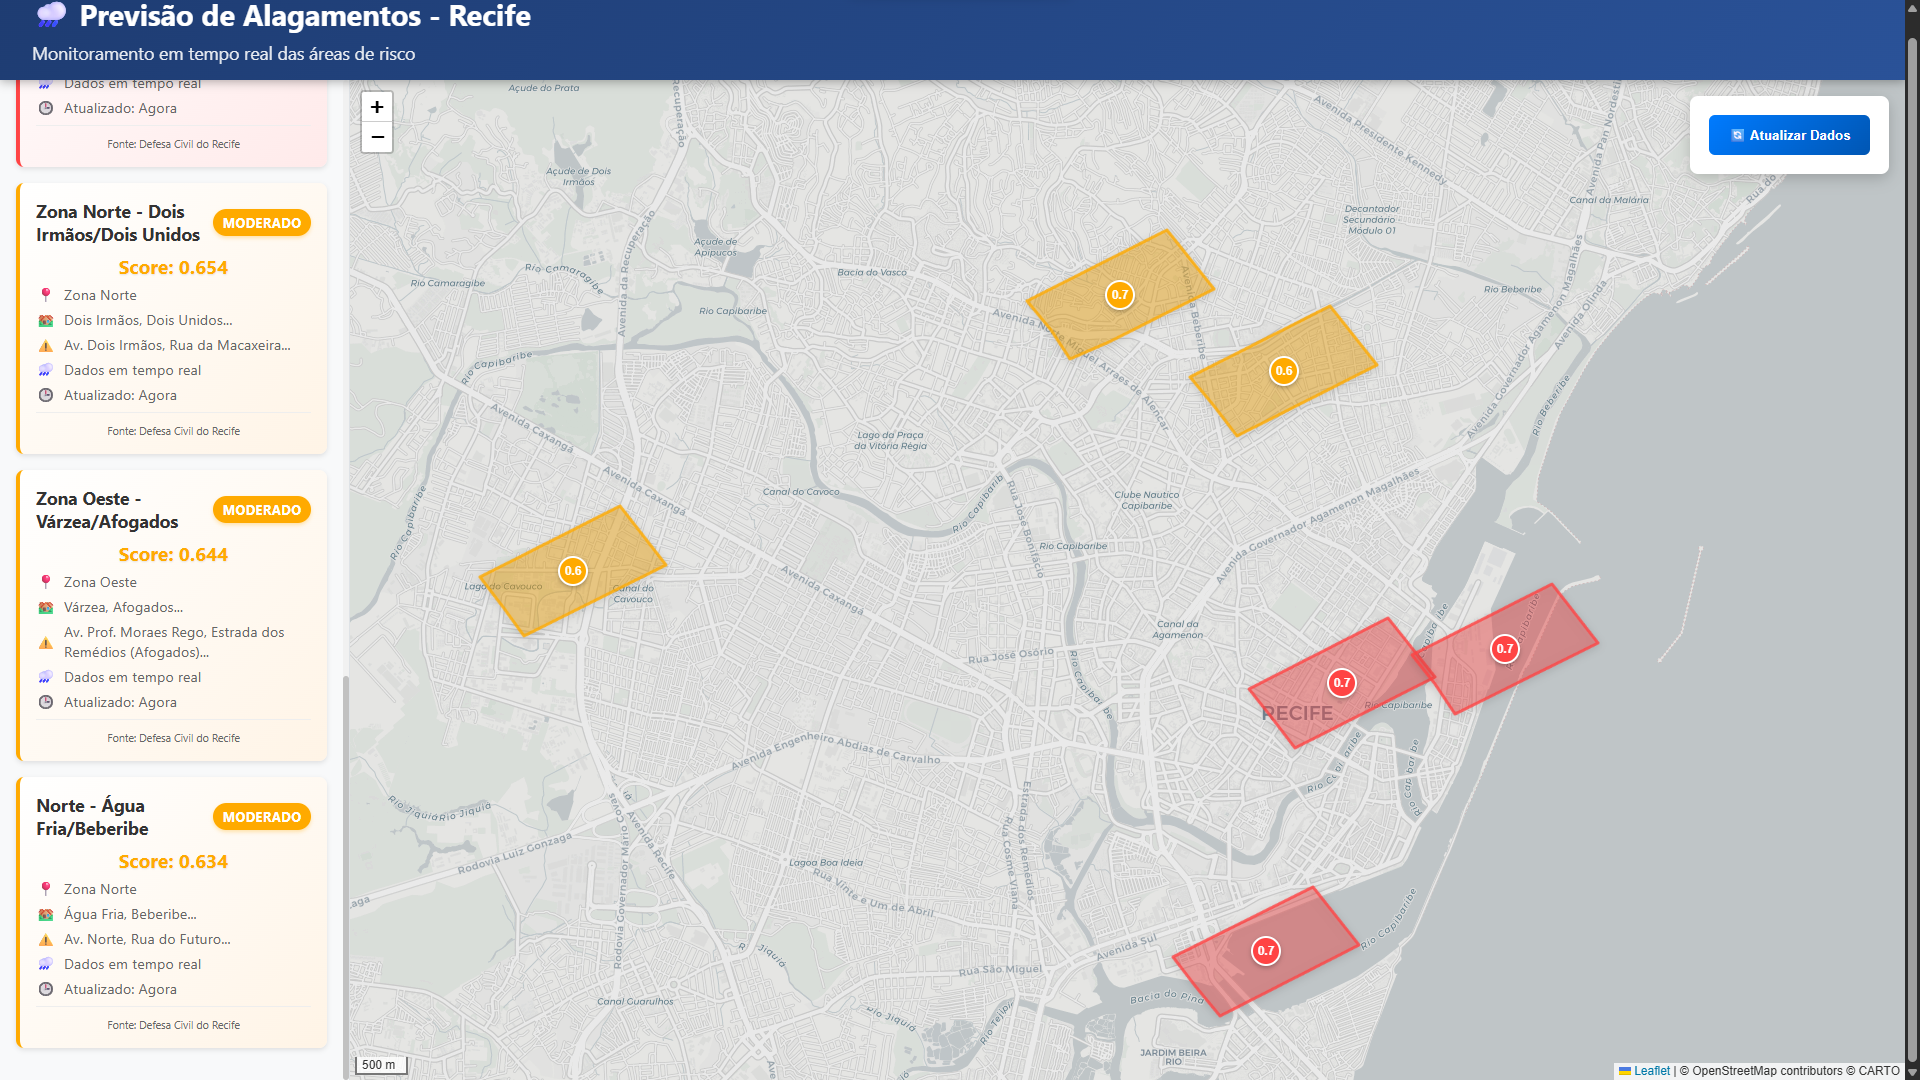
\includegraphics[width=0.9\textwidth]{figuras/dashboard.png}
  \caption{Mapa interativo exibindo áreas de risco no Recife}
  \label{fig:dashboard-mapa}
\end{figure}

\begin{figure}[H]
  \centering
  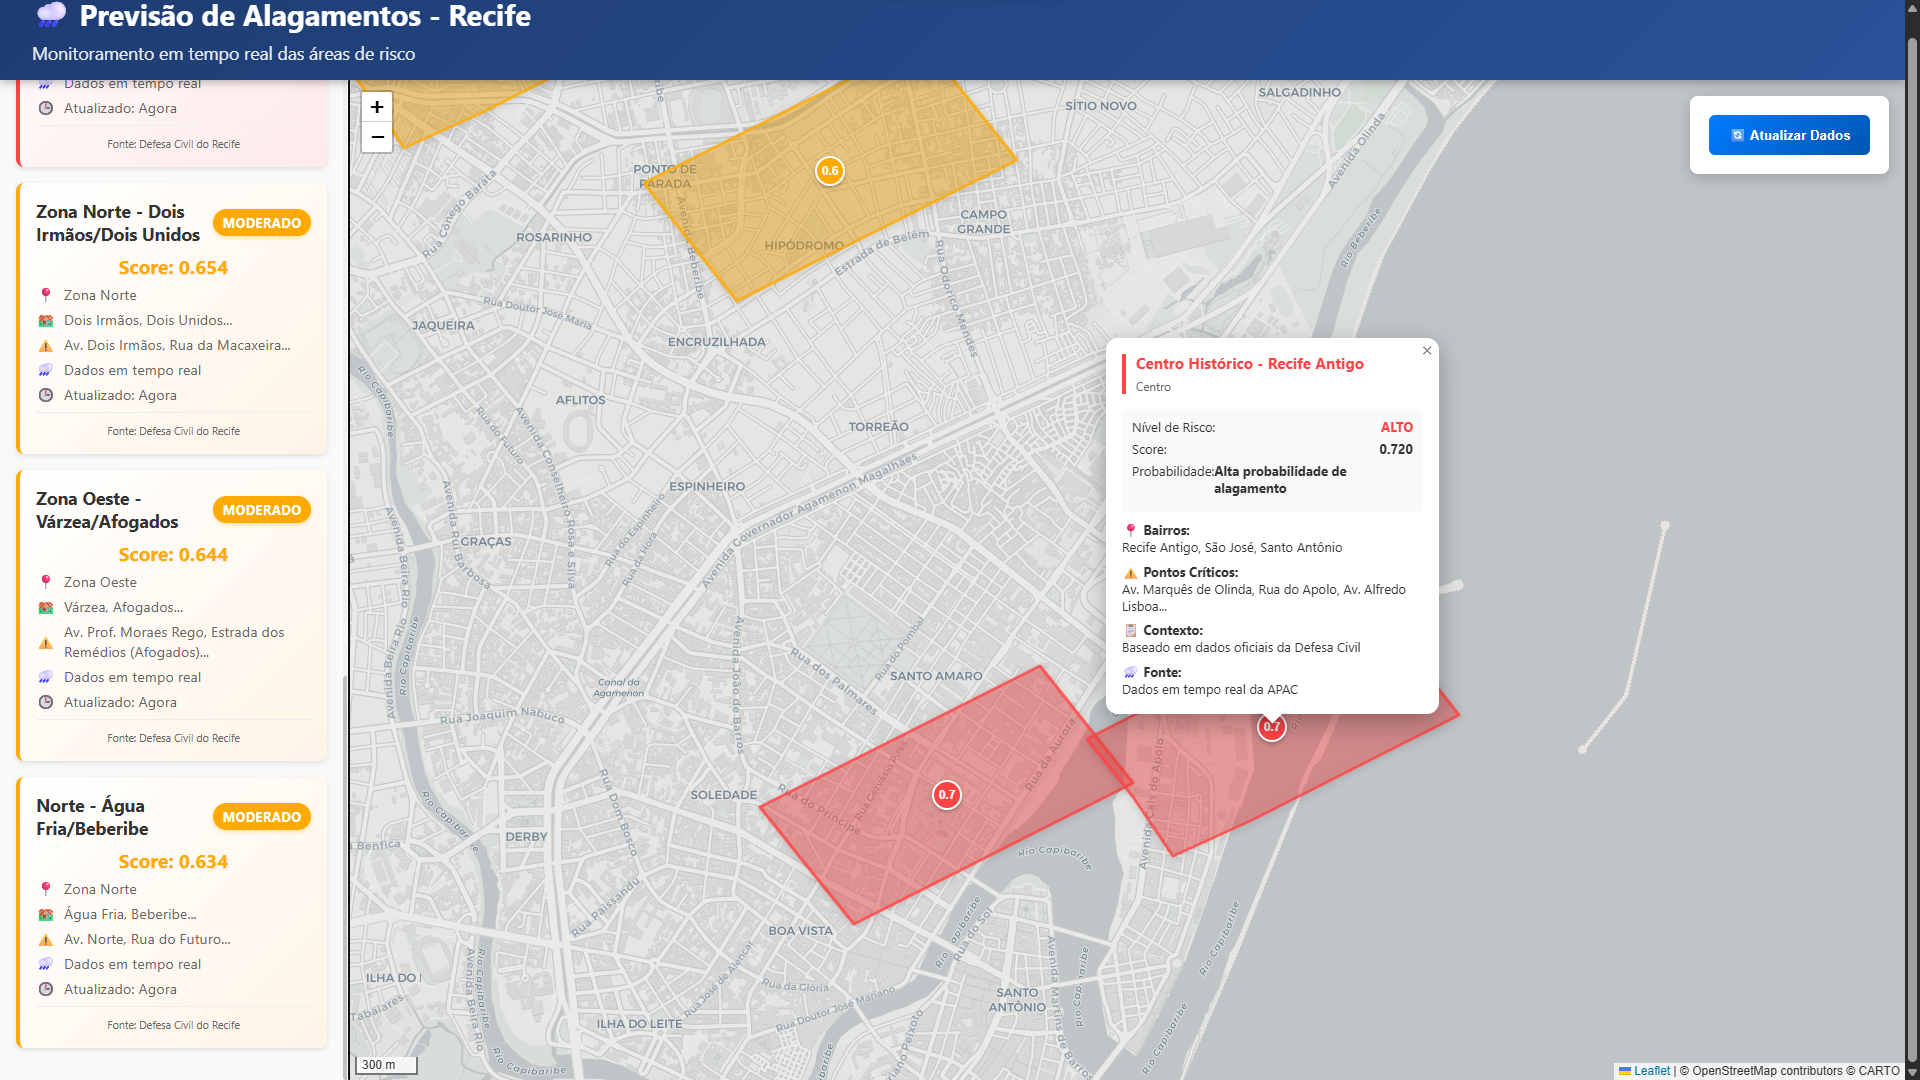
\includegraphics[width=0.9\textwidth]{figuras/dash-figura.png}
  \caption{Detalhes da região selecionada}
  \label{fig:dashboard-alertas}
\end{figure}


Essas visualizações permitem que tanto gestores públicos quanto cidadãos acompanhem em tempo real a evolução das chuvas e os riscos de alagamento, facilitando a tomada de decisão preventiva.
